%
%		    Modelo de TP gen�rico en LaTeX
%		    ~~~~~~~~~~~~~~~~~~~~~~~~~~~~~~
%		  Para la Facultad de Ingenier�a, UBA 
%
%		    Diego Essaya <dessaya@fi.uba.ar>
%
% Para compilar
% -------------
%
%   Este documento utiliza bastantes paquetes LaTeX. Si te falta alguno,
%   coment� la l�nea \useepackage{paquete} y prob� compilarlo de nuevo.
%
%   Si vas a usar este c�digo como base para crear tu TP, coment� todos los 
%   paquetes que no utilices. (Por ejemplo, si no vas a crear subfiguras, 
%   el paquete subfigure no es necesario).
% 
%   Formato DVI (necesario para convertir a PS y PDF):
%     $ latex tp-generico.tex
%
%     (repetir para que se generen las referencias cruzadas correctamente).
%
%   Formato PDF:
%     $ dvipdf tp-generico.dvi
% 
%     Normalmente podr�as compilar directamente en formato PDF con el 
%     comando pdflatex, pero este documento en particular incluye algunas 
%     im�genes que no pueden ser compiladas de esta forma, por lo que para 
%     generar un pdf se debe hacer el pasaje tex -> dvi -> pdf.
%

%
% Ac� se define el tama�o de letra principal:
%
\documentclass{article}

  

%
% T�tulo y autor(es):
%
\title{T�tulo del TP}
\author{Fulanito\\Menganito\\Pepito}

%------------------------- Carga de paquetes ---------------------------
%
% Si no necesit�s alg�n paquete, comentalo.
%

%
% Definici�n del tama�o de p�gina y los m�rgenes:
%
\usepackage[a4paper,headheight=16pt,scale={0.8,0.75},hoffset=0.5cm]{geometry}

%
% Vamos a escribir en castellano:
%
\usepackage[spanish, activeacute]{babel}
\usepackage[latin1]{inputenc}

%
% Si prefer�s el tipo de letra Helvetica (Arial), descoment� las siguientes
% dos lineas (las f�rmulas seguir�n estando en Times):
%
%\usepackage{helvet}
%\renewcommand\familydefault{\sfdefault}

%
% El paquete amsmath agrega algunas funcionalidades extra a las f�rmulas. 
% Adem�s defino la numeraci�n de las tablas y figuras al estilo "Figura 2.3", 
% en lugar de "Figura 7". (Por lo tanto, aunque no uses f�rmulas, si quer�s
% este tipo de numeraci�n dej� el paquete amsmath descomentado).
%
\usepackage{amsmath}
\numberwithin{equation}{section}
\numberwithin{figure}{section}
\numberwithin{table}{section}

%
% Para tener cabecera y pie de p�gina con un estilo personalizado:
%
\usepackage{fancyhdr}

%
% Para poner el texto "Figura X" en negrita:
% (Si no ten�s el paquete 'caption2', prob� con 'caption').
%
\usepackage[hang,bf]{caption}

%
% Para poder usar subfiguras: (al estilo Figura 2.3(b) )
%
\usepackage{subfigure}

%
% Para poder agregar notas al pie en tablas:
%
\usepackage{threeparttable}
\usepackage{multirow}
\usepackage{placeins}
\usepackage{float}
\usepackage{lscape}
%------------------------------ graphicx ----------------------------------
%
% Para incluir im�genes, el siguiente c�digo carga el paquete graphicx 
% seg�n se est� generando un archivo dvi o un pdf (con pdflatex). 
%
\newif\ifpdf
\ifx\pdfoutput\undefined
	\pdffalse
\else
	\pdfoutput=1
	\pdftrue
\fi

\ifpdf
	\usepackage[pdftex]{graphicx}
	\pdfcompresslevel=9
\else
	\usepackage[dvips]{graphicx}
\fi

%
% Todas las im�genes est�n en el directorio tp-img:
%
\newcommand{\imgdir}{tp-img}
\graphicspath{{\imgdir/}}
%
%------------------------------ graphicx ----------------------------------

\usepackage{wrapfig}

%------------------------- Inicio del documento ---------------------------
\usepackage{moreverb}
\usepackage{alltt}
\usepackage{fontenc}
\textheight=23.94cm
\textwidth=17cm 
\begin{document}
\Large

%
% Hago que en la cabecera de p�gina se muestre a la derecha la secci�n,
% y en el pie, en n�mero de p�gina a la derecha:
%
\pagestyle{fancy}
\renewcommand{\sectionmark}[1]{\markboth{}{\thesection\ \ #1}}
\renewcommand{\footrulewidth}{0.6pt} % Ancho de la línea horizontal sobre el pie (que en este ejemplo está vacío)

\lhead{Simulaci\'on de Sistemas}
\chead{}
\rhead{\rightmark}
\lfoot{}
\cfoot{\thepage}
\rfoot{ITBA}

%
% Car�tula:
%
\begin{titlepage}

%
% Sin cabecera ni pie de p�gina:
%
	%\thispagestyle{Empty}
%
% Logo de la facu arriba a la izquierda: 
	
	\begin{figure}
\begin{center}
%\includegraphics[width=6cm]{iag.jpg}
%	\includegraphics{fluxmed1.jpg}
	\end{center}
\end{figure}

\vspace{3cm}
% T�tulo:
%
	\begin{center}
		\underline{\Huge{Final de Simulaci\'on de Sistemas}}\\
\vspace{1cm}
	    \huge{Instituto Tecnol\'ogico de Buenos Aires
		\vspace{1cm}
		
}	\end{center}
	\vspace{1.5cm}
%
% Integrantes:
%


\noindent \huge{{\bf}
\\
\Large{{\bf Profesor:}} Alejandro Diaz. \\
\\
  \Large{{\bf Al'umnos:}}
\begin{itemize}
 \item Lucila Stancato \\
\item Conrado Negro \\
\item Damian Modernell \\
\item Juan Brasca 

\end{itemize}
 

	\vfill
% Fecha o cuatrimestre:
  \begin{center}
		\huge{14 de Diciembre de 2009}
	\end{center}
%	\flushright{\Large{ Junio 2009}}
}
\end{titlepage}


%
% Hago que las p�ginas se comiencen a contar a partir de aqu�:
%
\setcounter{page}{1}

%
% Pongo el �ndice en una p�gina aparte:
%
\tableofcontents
\newpage

%
% Inicio del TP:
%

\newpage
\section{Resoluci\'on}

\subsection*{a)}

\subsubsection*{Tiempo entre arribos al sistema}
Mediante mediciones del horario de arribo de clientes al sistema, computamos
los intervalos de tiempo entre arribos, y los representamos en el histograma
de la figura 1. Est\'a dividido en 7 intervalos de clase determinados a partir
de la f\'ormula de Sturgess que observamos en la ecuaci\'on 1.1.

\begin{equation}
 k = 1 + 3.3 * Log(n)
\end{equation}
donde $k$ es el N$^o$ de intervalos y $n$ es el N$^o$ de muestras.

\begin{figure}
\begin{center}
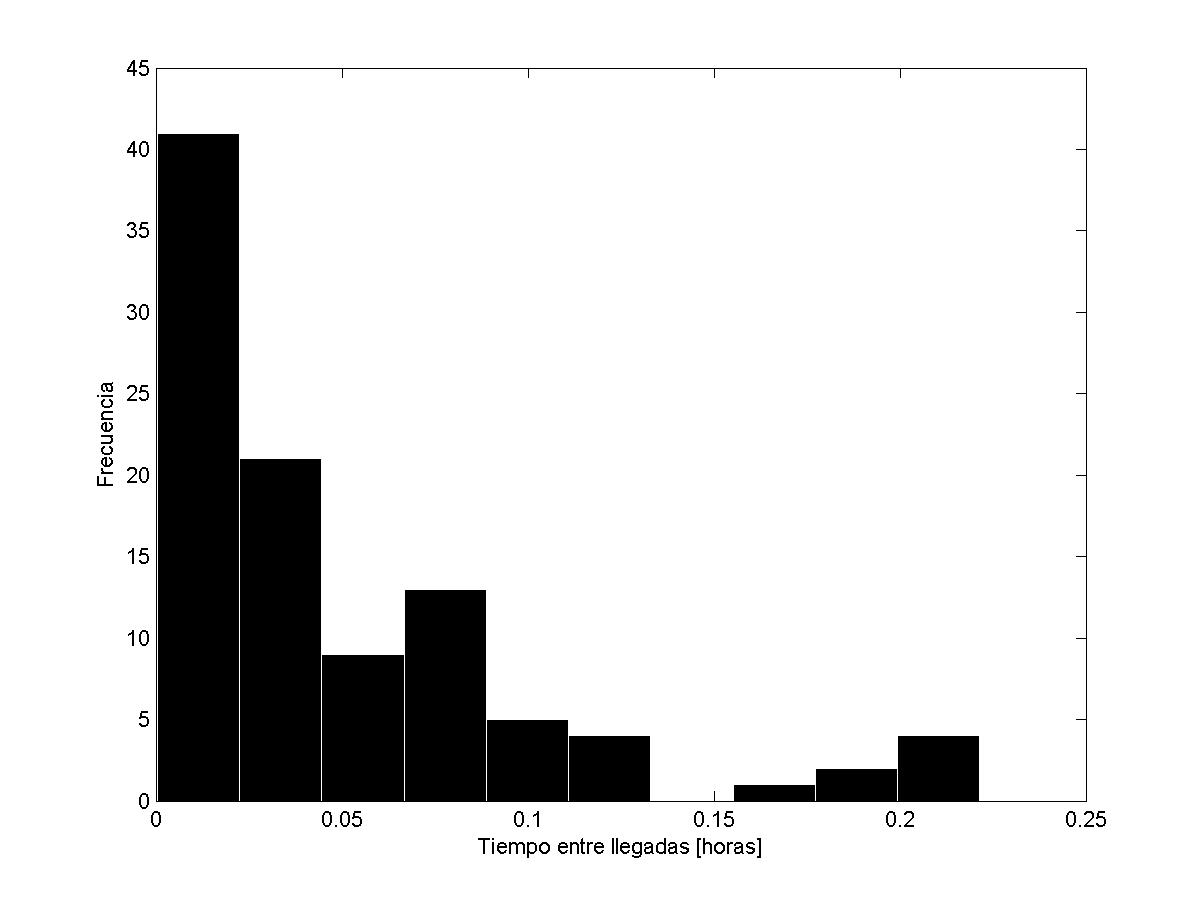
\includegraphics[width=11cm]{histograma_llegadas}
\caption{Histograma de intervalos de tiempo entre arribos de clientes al sistema. Se puede observar que parece provenir de una variable aleatoria con distribuci\'on exponencial.}
\end{center}
\end{figure}

Para determinar si la distribuc\'on de probabilidad del tiempo entre arribos
de clientes al sistema es exponencial, realizamos el test de bondad de ajuste
$\chi^2$. Las hip\'otesis del test son:

\begin{itemize}
 \item {$H_{0}$:} $\chi_{0}^2 < \chi_{n-1,\alpha}$ (Las llegadas de clientes al sistema est\'an exponencialmente distribuidas)
 \item {$H_{1}$:} $\chi_{0}^2 \ge \chi_{n-1,\alpha}$ (Las llegadas de clientes al sistema NO est\'an exponencialmente distribuidas)
\end{itemize}

A partir de las mediciones y de los valores esperados para cada
intervalo de clase, computamos el estad\'istico $\chi_{0}^2 = 10.709$. Como el valor
cr\'itico con un nivel de significaci\'on de 5\% y con 5 grados de libertad resulta 
$\chi_{0.05,5}^2 = 11.07$, rechazamos $H_1$ en favor de $H_0$.

\subsubsection*{Tasa de servicio de la estaci\'on $E3$}
Analizamos los tiempos de servicio de la estaci\'on $E3$ medidos del sistema, y volcamos
los datos a un histograma (ver figura 2) de 8 intervalos de clase tambi\'en computados
a partir de la f\'ormula de Sturgess.

\begin{figure}
\begin{center}
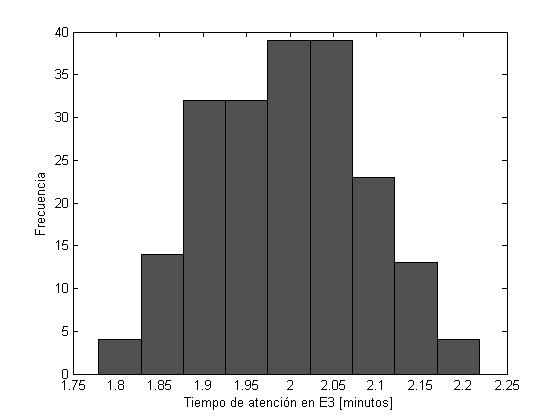
\includegraphics[width=11cm]{histograma_e3}
\caption{Histograma de la medici\'on de los tiempos de servicio del servidor $E3$. Observamos que los datos parecen provenir de una variable aleatoria con distribuci\'on normal.}
\end{center}
\end{figure}

En la figura 2, observamos que los datos parecen provenir de una variable aleatoria con distribuci\'on normal.
Para poder determinar si esto es cierto, realizamos el test estad\'istico $\chi^2$ con las siguientes hip\'otesis:

\begin{itemize}
 \item {$H_{0}$:} $\chi_{0}^2 < \chi_{n-1,\alpha}$ (El tiempo de servicio de la estaci\'on $E3$ es una variable aleatoria con distribuci\'on normal)
 \item {$H_{1}$:} $\chi_{0}^2 \ge \chi_{n-1,\alpha}$ (El tiempo de servicio de la estaci\'on $E3$ NO es una variable aleatoria con distribuci\'on normal)
\end{itemize}

Estimamos la media y la varianza de la distribuci\'on resultando:
\begin{itemize}
 \item {$\mu$ =} $1.995$
 \item {$\sigma^2$ =}  $0.008332$
\end{itemize}

El valor del estad\'istico resulta $\chi_{0}^2 = 4,7492$, y como el valor
cr\'itico es $\chi_{5,0.05}^2 = 11.07$ se rechaza $H_1$ en favor de $H_0$.

\subsection{b)}

\subsection{c)}

\subsection{d)}

\subsection{e)}


\begin{thebibliography}{1}
\bibitem{IEEhowto:kopka}
http://es.wikipedia.org/wiki/Regla\_de\_Sturgess
\end{thebibliography}


\end{document}

